\documentclass[a4paper]{article}
\usepackage[utf8]{inputenc}
\usepackage[spanish, es-tabla, es-noshorthands]{babel}
\usepackage[table,xcdraw]{xcolor}
\usepackage[a4paper, footnotesep = 1cm, width=20cm, top=2.5cm, height=25cm, textwidth=18cm, textheight=25cm]{geometry}
%\geometry{showframe}

\usepackage{tikz}
\usepackage{amsmath}
\usepackage{amsfonts}
\usepackage{amssymb}
\usepackage{float}
\usepackage{graphicx}
\usepackage{caption}
\usepackage{subcaption}
\usepackage{multicol}
\usepackage{multirow}
\setlength{\doublerulesep}{\arrayrulewidth}
\usepackage{booktabs}

\usepackage{hyperref}
\hypersetup{
    colorlinks=true,
    linkcolor=blue,
    filecolor=magenta,      
    urlcolor=blue,
    citecolor=blue,    
}

\newcommand{\quotes}[1]{``#1''}
\usepackage{array}
\newcolumntype{C}[1]{>{\centering\let\newline\\\arraybackslash\hspace{0pt}}m{#1}}
\usepackage[american]{circuitikz}
\usetikzlibrary{calc}
\usepackage{fancyhdr}
\usepackage{units} 

\graphicspath{{../Ejercicio-1/}{../Ejercicio-2/}{../Ejercicio-3/}{../Ejercicio-4/}}

\pagestyle{fancy}
\fancyhf{}
\lhead{22.01 Teoría de Circuitos}
\rhead{Mechoulam, Lambertucci, Rodriguez Turco, Londero, Galdeman}
\rfoot{\centering \thepage}
\begin{document}

\subsection{Introducción}
Con certeza, es posible afirmar que la onda senoidal es una de las formas de onda fundamentales tanto en el sentido matemático, puesto que cualquier otra forma de onda se puede expresar como una combinación de Fourier de ondas senoidales básicas, como en el
sentido práctico, debido a que se usa en forma extensiva como señal de prueba, de referencia
y como portadora. A pesar de su simplicidad, su generación resulta una tarea demandante si
se desea estar cerca de la pureza. Asimismo, los circuitos de amplificadores operacionales que han obtenido
mayor prominencia en la generación de ondas senoidales son el oscilador de puente de Wien
y el oscilador de cuadratura, de los cuales a continuación se expondrá únicamente el oscialdor de Wien.
\subsection{Oscilador Básico de puente de Wien.}
En el circuito de la figura (\ref{fig:wienbasico}) se emplea tanto retroalimentación negativa, a través de $R_2$
y $R_1$, como retroalimentación positiva, a través de los circuitos RC en serie y en paralelo.
Además, el comportamiento del circuito resulta muy afectado por la prevalencia de la retroalimentación positiva o negativa. Es necesario que los componentes de los circuitos RC
no tengan los mismos valores; sin embargo, si éstos se igualan, se simplifica el análisis.
El circuito se puede ver como un amplificador no inversor que amplifica a Vp en la
cantidad dada por la ecuación.
 \begin{align}
 A=\frac{V_0}{V_p}=1+\frac{R_2}{R_1}
 \end{align}

\begin{figure}[H]
	\centering
	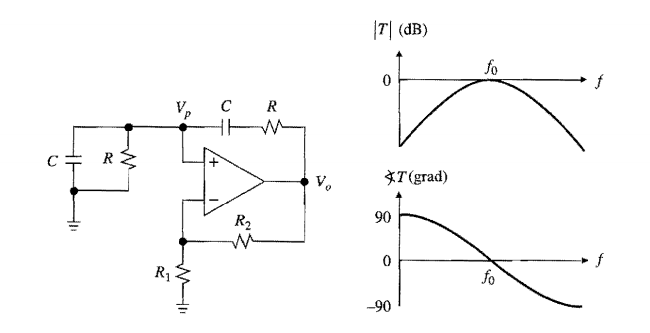
\includegraphics[width=0.7\textwidth]{Imagenes-Ej1/102.png}
	\caption{Circuito de puente de Wien y su lazo de ganancia T(jf) para el caso
	\label{fig:wienbasico}
$\frac{R_2}{R_1} =2$. }
\end{figure}
donde, por simplicidad, se supone un amplificador operacional ideal. Después, se sustituye Vp por el mismo amplificador operacional a través de los dos circuitos RC como:
\begin{align}
V_p= V_o \cdot \frac{Z_p}{Z_p+Z_s}
\end{align}
\begin{align}
Z_p= R \ // \frac{1}{j2\pi f C} \ \ \ \ R + \frac{1}{j2\pi f C} 
\end{align}
A partir de estas expresiones se puede despejar.
\begin{align}
\beta (jf)=\frac{V_p}{V_o}=\frac{1}{3+j\cdot \left( \frac{f}{f_0}-\frac{f_0}{f} \right) }
\end{align}
Donde $f_0 = \frac{1}{2\pi RC}$. La ganancia total experimentada por una señal al recorrer el lazo es
$T(jf)=A \cdot B$:
 \begin{align}
T (jf)=\frac{1+\frac{R_2}{R_1}}{3+j\cdot \left( \frac{f}{f_0}-\frac{f_0}{f} \right) }
\end{align}
La cual es una función pasa banda puesto que se aproxima a cero tanto en frecuencias altas
como en bajas. Su valor pico ocurre en $f= fo$ y es igual a
 \begin{align}
T (jf)=\frac{1+\frac{R_2}{R_1}}{3}
\label{eq:107}
\end{align}
El hecho de que $T(jf_o)$ sea real indica que una señal de frecuencia $fo$ experimentará un
cambio de fase neto de cero al recorrer el lazo. Dependiendo de la magnitud de $T(jf_o)$, se
tienen tres posibilidades distintas: 
\begin{enumerate}
\item  	$T(jf_o) < 1$, esto es, $A < 3 $. Cualquier perturbación de frecuencia $fo$ surgida en la
entrada del amplificador operacional, primero es amplificada por $A < 3$, y después por $B(jf_o) =\frac{1}{3}$,
para una ganancia neta menor de uno. La intuición indica que esta perturbación se reduce cada vez que recorre el lazo hasta que de manera eventual decae hasta cero. Así, es
posible establecer que la retroalimentación negativa (a través de R2 y R1) prevalece 
sobre la retroalimentación positiva (a través de Zs y Zp), lo que resulta en un sistema estable. En consecuencia, los polos del circuito descansan en la mitad izquierda del
plano complejo. 
\begin{figure}[H]
	\centering
	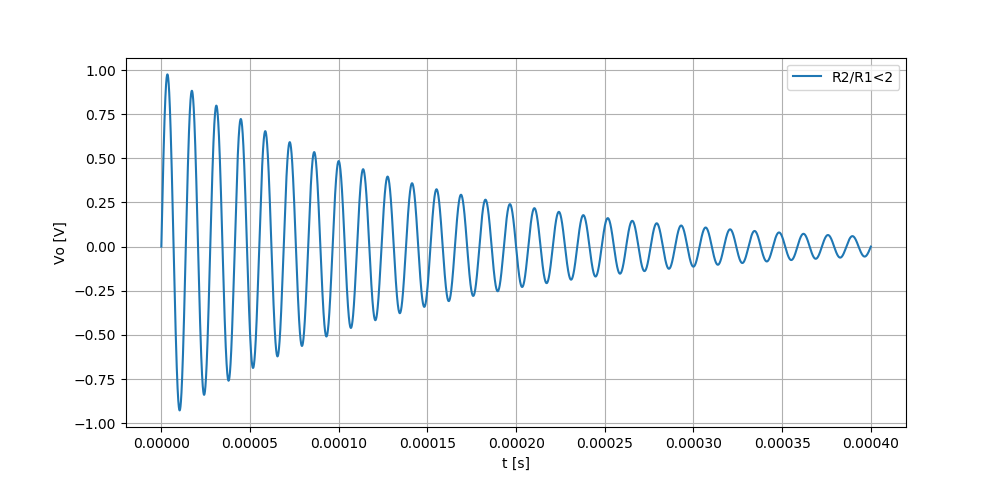
\includegraphics[width=\textwidth]{Imagenes-Ej1/r1r2m.png}
	\label{fig:r1r2m}
	\caption{$V_0 \implies \frac{R_2}{R_1}<2$}
\end{figure}
\item 	 $T(jf_o) > 1$, esto es, $A> 3$. Ahora la retroalimentación positiva prevalece sobre la
retroalimentación negativa, lo cual indica que una perturbación de frecuencia $fo$ se amplificará en forma regenerativa, ocasionando que el circuito rompa en oscilaciones de
magnitud creciente. Así, el circuito es inestable y sus polos descansan en la mitad derecha del plano complejo. Como es sabido, las oscilaciones se presentarán hasta que se
alcancen los límites de saturación del amplificador operacional. Después de eso, cuando se observe a Vo
con el osciloscopio aparecerá como una onda senoidal recortada.
\begin{figure}[H]
	\centering
	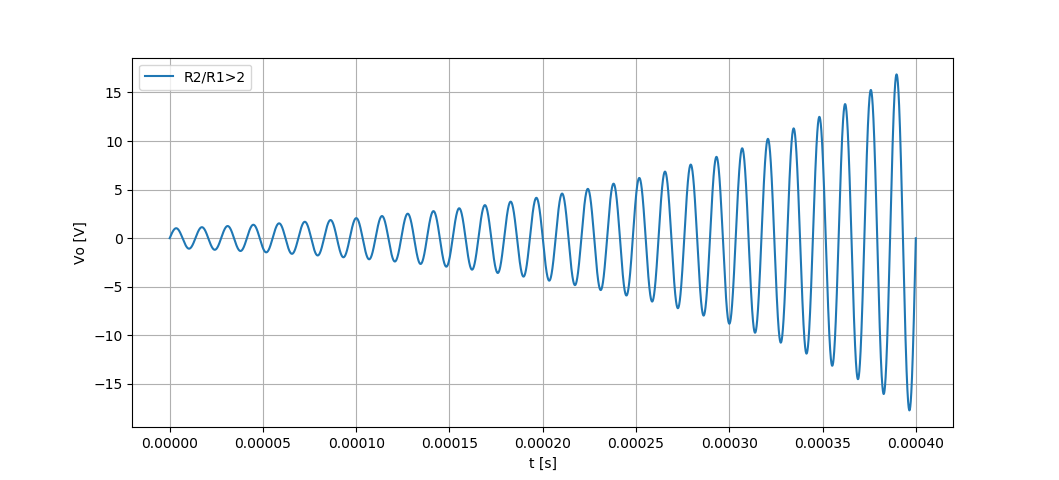
\includegraphics[width=\textwidth]{Imagenes-Ej1/r1r2g.png}
	\label{fig:r1r2g}
	\caption{$V_0 \implies \frac{R_2}{R_1}>2$}
\end{figure}
\item  $T(jf_o) = 1$, o bien $A= 3$ exactamente, esta condición se denomina como estabilidad
neutral, debido a que las retroalimentaciones positiva y negativa se aplican en cantidades iguales. Cualquier perturbación de frecuencia $fo$ primero es amplificada por 3  y
después por $\frac{1}{3}$ , lo cual indica que, una vez iniciada, se sostendrá en forma indefinida. Como es sabido, esto corresponde a un par de polo que está justo sobre el eje jw. Las
condiciones $\sphericalangle T(jf_0)= 0^\circ$ y $|T(jfo)|= 1$, en conjunto se denominan el criterio de
Barkhausen para la oscilación en $f=fo$. La naturaleza pasa banda de $T(jf)$ permite que la
oscilación ocurra sólo además, cualquier intento de oscilación en otras frecuencias se desalienta en forma natural debido a que ahí  $\sphericalangle T(jf_0) \neq 0^\circ$ y $|T(jf)| < 1$. Con base en la
ecuación (\ref{eq:107}), la estabilidad neutral se alcanza con 
\begin{align}
\frac{R_2}{R_1}=2
\end{align}
Resulta evidente que, cuando se cumple esta condicion, los componentes alrededor del amplificador operacional forman un puente balanceado en $f=f_0$.
\begin{figure}[H]
	\centering
	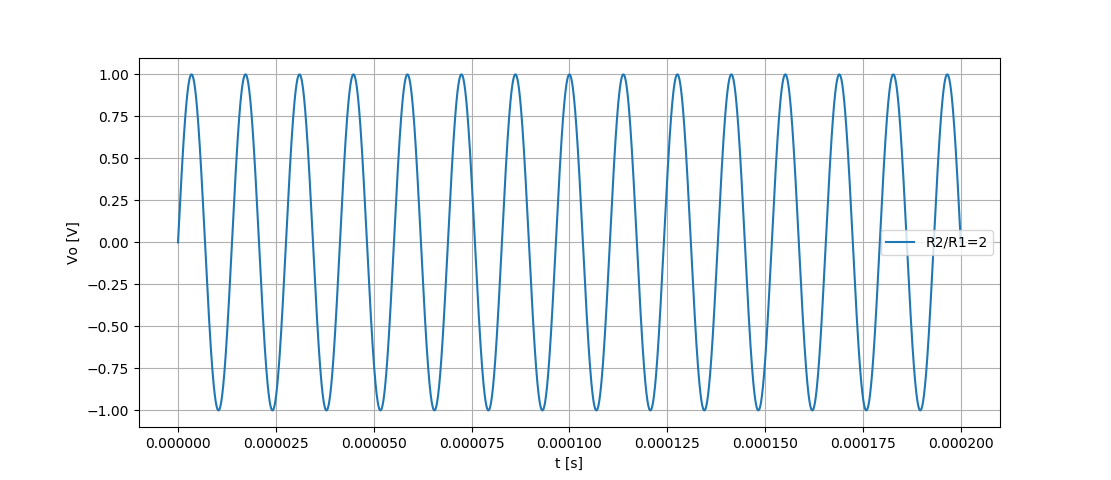
\includegraphics[width=\textwidth]{Imagenes-Ej1/r2r1e.png}
	\label{fig:r1r2e}
	\caption{$V_0 \implies \frac{R_2}{R_1}=2$}
\end{figure}
\end{enumerate}
Finalmente se obtiene la transferencia del circuito:
\begin{align}
H(s)=\frac{T(s)}{1-T(s)}\cdot \frac{1}{\beta}
\end{align}
En un circuito de la vida real, la dispersión de los componentes hace difícil mantener al
puente balanceado de manera exacta. Además, se deben tomar precauciones: 
\begin{itemize}
\item Para que la
oscilación inicie en forma espontánea al encender el circuito.
\item Para que su amplitud se
mantenga por debajo de los límites de saturación del amplificador operacional y así evitar la distorsión excesiva.

\end{itemize}

 Estos objetivos se satisfacen haciendo que la relación $\frac{R_2}{R_1}$ sea dependiente de la
amplitud, de manera que en los niveles bajos de señal ésta sea sólo un poco mayor que 2
para asegurar que la oscilación inicie, y en los niveles altos de señal ésta sea sólo un poco
menor que 2 para limitar la amplitud. Entonces, una vez que la oscilación ha iniciado, ésta
crecerá y se estabilizará de forma automática en algún nivel intermedio donde $\frac{R_2}{R_1}=2$
exactamente.\\
La estabilización de la amplitud toma muchas formas, todas las cuales utilizan elementos no lineales para reducir $R_2$ o incrementar $R_1$ junto con la amplitud de la señal. Para
proporcionar una base intuitiva a esta exposición, se continuará usando la función $T(jf)$,
pero en un sentido \emph{\textbf{incremental}} debido a la no linealidad que ahora presenta el circuito, se utilizó el siguiente circuito.\\
\begin{figure}[H]
	\centering
	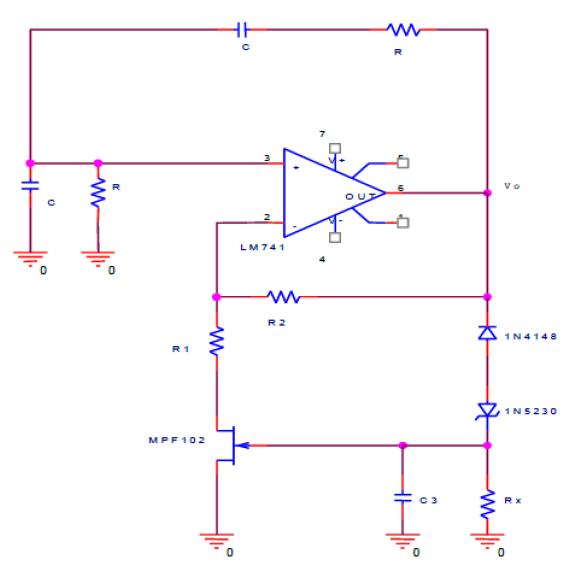
\includegraphics[width=0.5\textwidth]{Imagenes-Ej1/oscCatedra.png}
	\label{fig:circosc}
	\caption{Circuito Oscilador de Wien con AGC.}
\end{figure}
Al encenderse el circuito, cuando el capacitor $C_3$ aún está descargado, el voltaje de gate está cerca de 0V, lo cual
indica una resistencia de canal baja. En efecto, el JFET acorta la resistencia de 51 k$\Omega$ a la
tierra para proporcionar $\frac{R_2}{R_1}>2$ , por lo tanto la oscilación
empieza a construirse. Los diodos y el capacitor $C_3$ forman un pico negativo, cuyo
voltaje se vuelve cada vez más negativo conforme crece la oscilación. Lo anterior reduce en
forma gradual la conductividad del JFET, ya que en el límite de corte completo se tendría $\frac{R_2}{R_1}<2$. Sin embargo, la amplitud se estabiliza en forma automática en
algún punto intermedio donde $\frac{R_2}{R_1}=2$ exactamente. Si el voltaje Gate Source correspondiente se denota como $V_{GS_{crit}}$, y la amplitud pico de salida como $V_{om}$ se tiene que $-V_{om} =V_{GS_{crit}} - V_{Don}$ Por ejemplo, con $VGS(crit) = -4.3$ se tiene que $Vom \approx 4.3 + 0.7 = 5 V$
En este caso se utilizó un JFET canal n, si se quisiera implementar con canal p bastaría con invertir los sentidos de ambos diodos para que la tensión del gate sea positiva y el control se haría en los semiciclos positivos.\\

\subsection{Elecciones de diseño.}
Para las consideraciones de diseño ($f_0 = 72.5 kHz$) que se deben cumplir se eligieron . \begin{itemize}
\item$C=1nF$
\item$R=2.195k\Omega$
\end{itemize} 

La red RC es la que se encarga de controlar la tensión del gate, y por lo tanto la ganancia del circuito. $C_3$ se carga cuando los diodos se activan en el hemiciclo negativo aumentando la tensión  del Gate , y se descarga en el hemiciclo positivo a a través de $R_X$. Es importante que la constante de tiempo para la carga del capacitor ($\tau=C_3R_X$ ) sea mucho mayor al periodo de la señal ($\approx 14\mu s$) para mantener la tensión a la salida. Además, para mantener esta tensión se necesita que $R_X$ sea lo suficientemente grande para que el capacitor no se descargue rápido, pero por otra parte el capacitor se tiene que poder descargar frente a variaciones en la
tensión de salida para poder ajustar la ganancia.
A partir de esto, se tomaron los siguientes valores:
\begin{align}
R_X=1M\Omega \ \ \ C=1\mu F
\end{align}

\subsection{JFET}
El transistor a utilizar es el MPF102. El rango de operación es en la zona lineal, la resistencia dinámica, rd, varía en un rango según la tensión del gate. Ésta resistencia se encuentra en
serie con $R_1$, por lo que cuando varía, también varía la ganancia del lazo.
\begin{align}
\frac{R_2}{R_1 \pm \Delta rd}
\end{align}
de aquí se obtiene que $R_2>2\cdot R_1$, Asi que se tomó $R_2=100k\Omega$ y para $R_1$ se utilizará una resistencia de 43k$\Omega$ junto a un preset de 10k$\Omega$ para poder ajustar la ganancia del lazo.
Se simularon las curvas características del transistor para distintos valores de tensión de gate:
\begin{figure}[H]
	\centering
	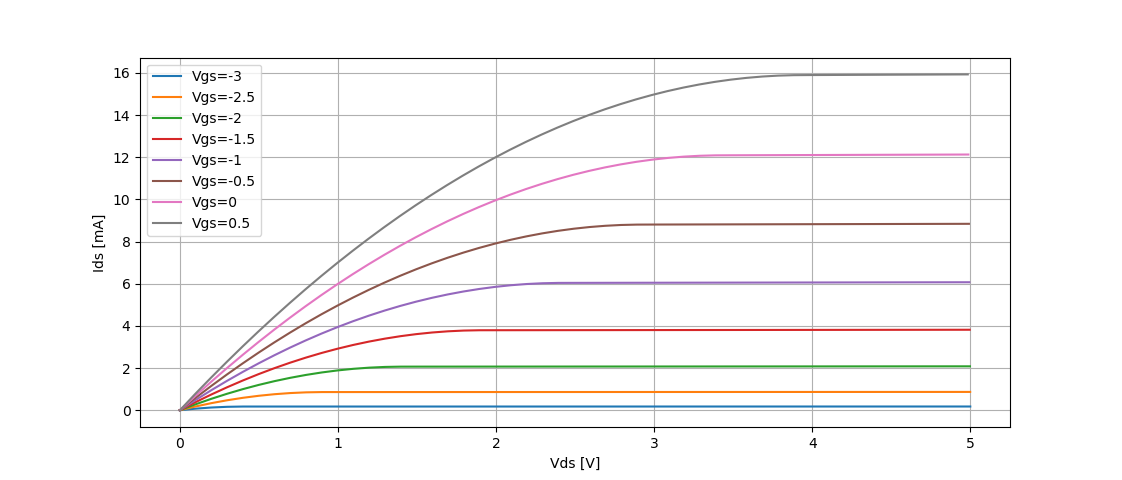
\includegraphics[width=\textwidth]{Imagenes-Ej1/curvasJfet.png}
	\label{fig:caracdcurv}
	\caption{Curvas características JFET}
\end{figure}

\subsection{Singularidades.}
Se realizaron diagramas de polos y ceros para $H(s)$ como para $T(s)$ en función de la variación de rd, obteniendo lo siguientes gráficos:
\begin{figure}[H]
	\centering
	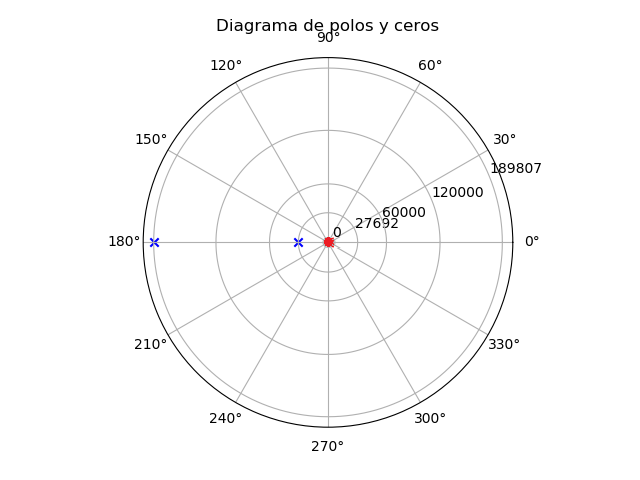
\includegraphics[width=0.5\textwidth]{Imagenes-Ej1/Tr=1.png}
	\label{fig:poleZeroDiagTs}
	\caption{Diagrama Polos y Ceros T(s)}
\end{figure}
\begin{figure}[H]
	\centering
	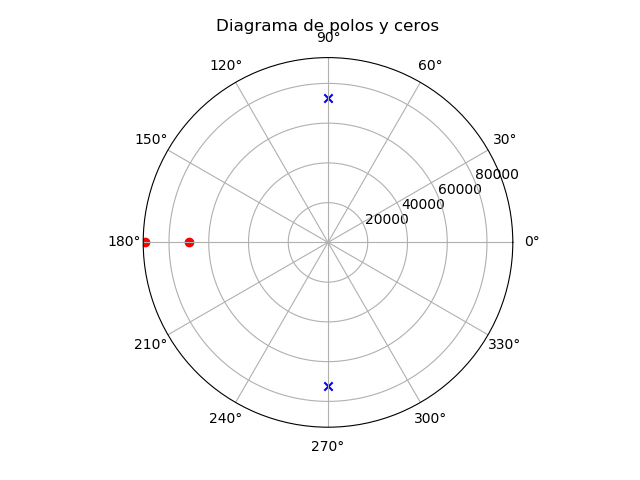
\includegraphics[width=0.5\textwidth]{Imagenes-Ej1/Hr=1.png}
	\label{fig:poleZeroDiagHs1}
	\caption{Diagrama Polos y Ceros H(s) con $\frac{R_2}{R_1}=2$}
\end{figure}
\begin{figure}[H]
	\centering
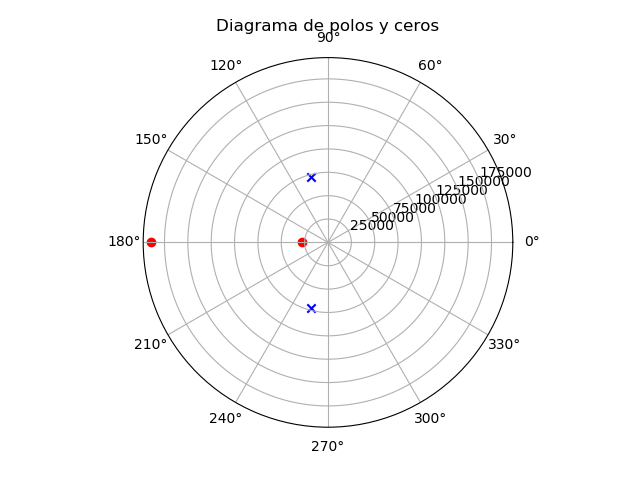
\includegraphics[width=0.5\textwidth]{Imagenes-Ej1/Hrmin1.png}
	\label{fig:poleZeroDiagHsmin}
	\caption{Diagrama Polos y Ceros H(s) con $\frac{R_2}{R_1}<2$}
\end{figure}
\begin{figure}[H]
	\centering
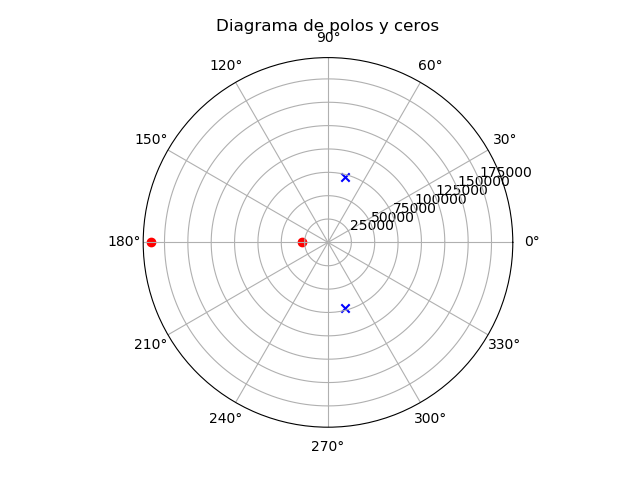
\includegraphics[width=0.5\textwidth]{Imagenes-Ej1/Hrmn1.png}
	\label{fig:poleZeroDiagHsmax}
	\caption{Diagrama Polos y Ceros H(s) con $\frac{R_2}{R_1}>2$}
\end{figure}
\subsection{Elección operacional.}

La exactitud y la estabilidad de la oscilación, al igual que la dinámica del amplificador operacional, resultan
afectadas por la calidad de los componentes pasivos. Los capacitores  y 
resistores SMD  son buenas elecciones para los elementos en el circuito de
retroalimentación positiva. En la práctica, con el fin de compensar para las tolerancias de
los componentes, en la práctica los circuitos de puente de Wien con frecuencia están equipados con correctores adecuados para el ajuste exacto de $f_o$, aquí utilizaremos un preset sobre una de las R para ajustar dicho $f_0$. 
Para evitar los efectos limitantes del slew-rate para una determinada
amplitud pico de salida $V_{om}$ el amplificador operacional debe tener $SR > 2\pi V_{om} f_o$. Una vez que esta
condición es cumplida, el factor limitante se convierte en el GBP finito, cuyo efecto es
una reducción de la frecuencia real de la oscilación. Es posible comprobar que para
mantener este cambio dentro del $10\%$ cuando se utiliza un amplificador operacional de GBP constante, éste
debe tener $GBP \approx 43 f_o$.
El extremo inferior del rango de frecuencia depende de qué tan grandes pueden hacerse los componentes en el circuito reactivo. Con el uso de amplificadores operacionales de entrada FET para
minimizar los errores de corriente de bias a la entrada, el valor de R se puede
incrementar fácilmente hasta el rango de decenas de megaohms. Por ejemplo, utilizando C =l $\mu$F Y R=15.9 M$\Omega$ se obtiene $f_o =0.01 Hz$.\\

Los amplificadores operacionales considerados son los siguientes:
\begin{table}[H]
\centering
\begin{tabular}{ccccccccc}
\textbf{Amplificador Operacional} & \textbf{GBP [Mhz]} & \textbf{SR [$\frac{V}{\mu s}$]} & \textbf{$Z_{in} [\Omega]$} & \textbf{$Z_{out}[\Omega]$} & \textbf{$I_{bias}[A]$} & \textbf{$I_{off}$[A]} & \textbf{$V_{off}$[mV]} & \textbf{THD} \\ \hline
\textit{TL-082}                   & 3                  & 13                              & 1T                         & -                          & 30p                 & 5p                    & 3                      & 0.003$\%$    \\
\textit{LM324}                    & 1                  & 0.3                             & -                          & -                          & 45                  & 5                     & 2                      & -            \\
\textit{LM833}                    & 10                 & 5                               & -                          & 37                         & 300n                & 10n                   & 0.3                    & 0.002$\%$    \\
\textit{LF356}                    & 2.5                & 12                              & 1T                         & -                          & 20p                 & 50p                   & 3                      & -            \\
\textit{LM741}                    & 1.5                & 0.5                             & 2M                         & 75                         & 80n                 & 20n                   & 2                      & -            \\
\textit{NE5534}                   & 10                 & 13                              & 100k                       & 0.3                        & 500n                & 20n                   & 0.5                    & -           
\end{tabular}
\end{table}

Considerando las restricciones para con el SR y GBP las mejores opciones son los operacionales \emph{TL082} ,\emph{LF356} y \emph{NE5534}, donde este ultimo fue descartado debido a su baja impedanica de entrada, y el LF356 debido a no contar con el dato de la distorsión armónica.
Finalmente queda el TL082 que es el que fue utilizado.
\subsection{Simulaciones}
\begin{figure}[H]
	\centering
	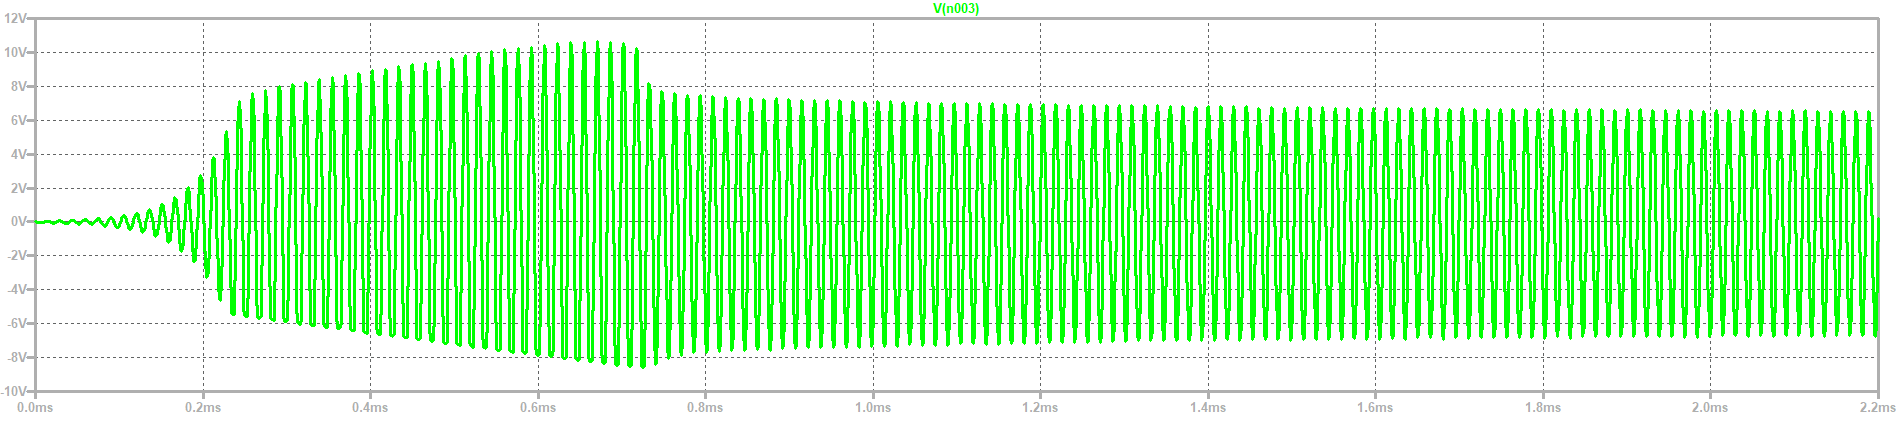
\includegraphics[width=\textwidth]{Imagenes-Ej1/trans.png}
	\caption{Respuesta transitoria}
	\label{fig:trans}

\end{figure}
\subsection{Conclusiones.}
%\begin{figure}[H]
%	\centering
%	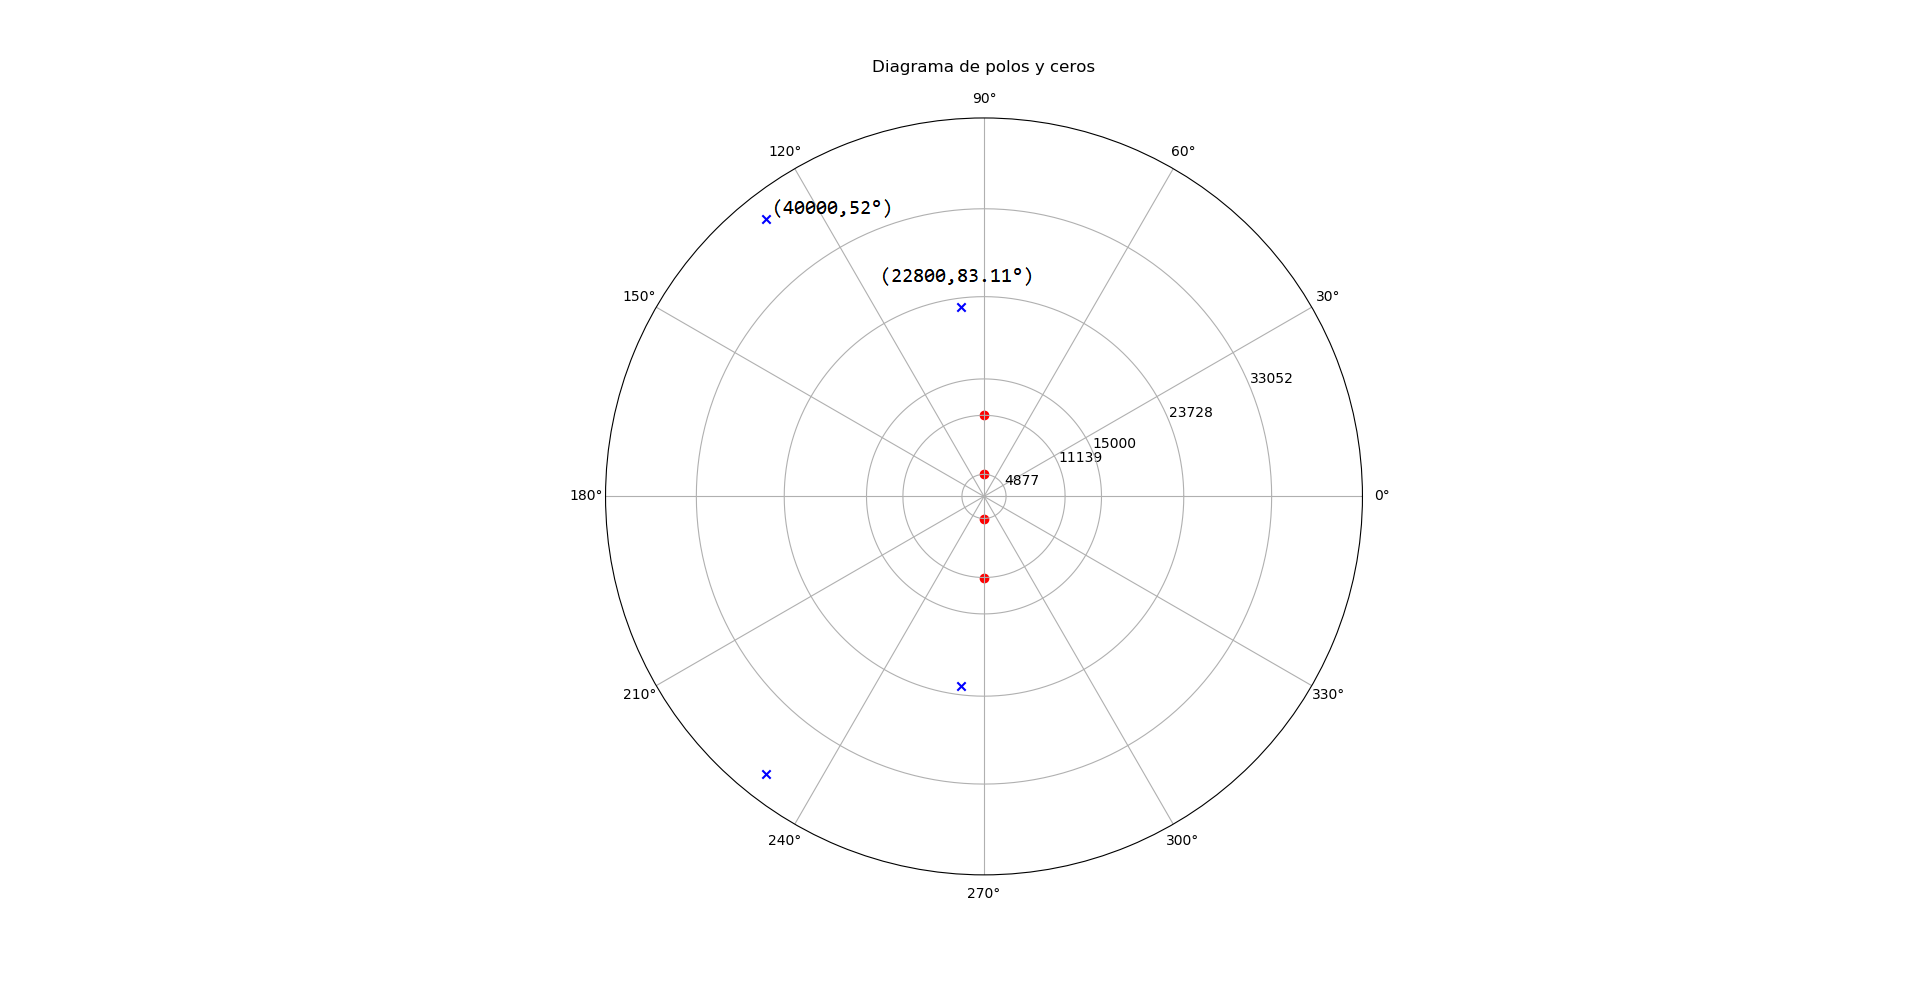
\includegraphics[width=\textwidth]{Imagenes-Ej3/DiagramaPolosYCeros.png}
%	\label{fig:poleZeroDiag}
%	\caption{Diagrama Polos y Ceros}
%\end{figure}
\end{document}